%======================================================================
\part{Fundamentos de la respuesta \'optica\\y Seminario I}
%======================================================================

\chapter{El problema cient\'ifico}
\label{ch:problema}

\section{Motivaci\'on}

Cuando la radiaci\'on electromagn\'etica atraviesa o refleja en un s\'olido, el material no responde de manera instant\'anea ni local en el sentido microsc\'opico m\'as general.
Macrosc\'opicamente, sin embargo, esa respuesta puede condensarse en unas pocas funciones de frecuencia.
Entre ellas, la funci\'on diel\'ectrica compleja es el objeto central:
contiene la informaci\'on sobre polarizaci\'on, absorci\'on, retardos de fase y, en \'ultima instancia, sobre excitaciones electr\'onicas, fonones, excitones y portadores libres~\cite{electrodynamics,MarkFox}.

El experimentalista suele medir una sola magnitud proyectada:
reflectividad a incidencia normal~$R(\omega)$,
coeficiente de absorci\'on~$\alpha(\omega)$,
transmitancia de una l\'amina~$T(\omega)$,
o bien el \'indice~$n$ y la extinci\'on~$k$ en un intervalo limitado.
El problema inverso consiste en reconstruir $\hat\varepsilon(\omega)$ ---y con ella el resto del espectro \'optico--- sin imponer un modelo microsc\'opico r\'igido del tipo Lorentz, Tauc--Lorentz o Fano, que puede sesgar la interpretaci\'on cuando la muestra no cabe en esas formas.

\section{Planteamiento formal}

En un medio lineal, homog\'eneo e is\'otropo (redes c\'ubicas, por simplicidad), el desplazamiento el\'ectrico y el campo el\'ectrico se relacionan en el dominio de Fourier por
\begin{equation}
\mathbf{D}(\omega)=\hat\varepsilon(\omega)\,\mathbf{E}(\omega),
\qquad
\hat\varepsilon(\omega)=\varepsilon_1(\omega)+i\varepsilon_2(\omega).
\end{equation}
La conductividad \'optica compleja $\hat\sigma(\omega)=\sigma_1(\omega)+i\sigma_2(\omega)$ es equivalente, en unidades gaussianas,
\begin{equation}
\label{eq:eps-sigma}
\hat\varepsilon(\omega)=1+\frac{4\pi i}{\omega}\hat\sigma(\omega).
\end{equation}
La causalidad ---el material no responde antes de que llegue el campo--- implica que $\varepsilon_1$ y $\varepsilon_2$ no son independientes: quedan ligados por las relaciones de Kramers--Kronig~\cite{Jackson,electrodynamics}:
\begin{align}
\label{eq:kk1}
\varepsilon_1(\omega)-1
&=\frac{2}{\pi}\,\mathcal{P}\!\int_{0}^{\infty}
\frac{x\,\varepsilon_2(x)}{x^{2}-\omega^{2}}\,dx,\\
\label{eq:kk2}
\varepsilon_2(\omega)
&=-\frac{2\omega}{\pi}\,\mathcal{P}\!\int_{0}^{\infty}
\frac{\varepsilon_1(x)-1}{x^{2}-\omega^{2}}\,dx
+\frac{4\pi\sigma_{\mathrm{dc}}}{\omega}.
\end{align}
Aqu\'i $\mathcal{P}$ denota el valor principal de Cauchy y $\sigma_{\mathrm{dc}}$ es la conductividad continua.

Si se midiera $\varepsilon_2(\omega)$ en todo el eje, $\varepsilon_1$ quedar\'ia fijada.
En el laboratorio el eje es finito.
Lo que queda fuera de la ventana experimental se resume en un fondo de alta frecuencia $\varepsilon_\infty$, y lo que queda dentro debe parametrizarse de forma flexible pero causal.
Ese es el n\'ucleo del an\'alisis variacional restringido de Kuzmenko~\cite{constrained}.

\section{Objetivos}

\paragraph{Objetivo general.}
Formular y demostrar, paso a paso, un procedimiento f\'isico completo para modelar la funci\'on diel\'ectrica compleja a partir de espectros \'opticos medibles mediante an\'alisis variacional Kramers--Kronig restringido, e implementar ese procedimiento en una aplicaci\'on de an\'alisis espectral que permita validar la consistencia de los resultados.

\paragraph{Objetivos espec\'ificos.}
\begin{enumerate}[leftmargin=*]
\item Derivar, desde las ecuaciones de Maxwell, las constantes \'opticas relevantes y sus v\'inculos con $\hat\varepsilon$.
\item Exponer el an\'alisis variacional con base triangular y la minimizaci\'on por Levenberg--Marquardt.
\item Especificar c\'omo cada magnitud medible ($R$, $T$, $\alpha$, $n$, $k$, $\varepsilon_1$, $\varepsilon_2$) entra en el funcional $\chi^{2}$.
\item Validar que los resultados reconstruidos son f\'isicamente verdaderos en el sentido de causalidad, pasividad, reproducci\'on de datos y consistencia cruzada entre constantes.
\end{enumerate}

\section{Alcance}

Se trabaja en respuesta lineal, medios no magn\'eticos ($\mu=1$), incidencia normal desde el vac\'io y, salvo indicaci\'on contraria, muestras semi-infinitas o l\'aminas en aire con reflexiones m\'ultiples incoherentes.
No se tratan aqu\'i elipsometr\'ias anisotr\'opicas ni multicapas arbitrarias sobre sustrato.
La luminiscencia se discute solo como emisi\'on: su intensidad no es $\varepsilon_2$ y no define un par Kramers--Kronig.

\section{Organizaci\'on de la tesis}

La \textbf{Parte~I} desarrolla el marco electromagn\'etico y culmina en el Seminario~I.
La \textbf{Parte~II} detalla el m\'etodo variacional, el ajuste y la f\'isica de cada medida; culmina en el Seminario~II.
La \textbf{Parte~III} presenta criterios de verdad experimental y resultados de validaci\'on.


\chapter{Marco electromagn\'etico}
\label{ch:marco}

\section{Ecuaciones de Maxwell en medios}

En unidades gaussianas, las ecuaciones macrosc\'opicas leen~\cite{Jackson}
\begin{align}
\nabla\cdot\mathbf{D}&=4\pi\rho_{\mathrm{lib}},&
\nabla\cdot\mathbf{B}&=0,\\
\nabla\times\mathbf{E}&=-\frac{1}{c}\frac{\partial\mathbf{B}}{\partial t},&
\nabla\times\mathbf{H}&=\frac{4\pi}{c}\mathbf{J}_{\mathrm{lib}}
+\frac{1}{c}\frac{\partial\mathbf{D}}{\partial t}.
\end{align}
Para campos arm\'onicos $e^{-i\omega t}$ y constitutivas lineales
$\mathbf{D}=\hat\varepsilon\mathbf{E}$, $\mathbf{B}=\mathbf{H}$ (no magn\'etico) y $\mathbf{J}=\hat\sigma\mathbf{E}$,
se recupera la relaci\'on~\eqref{eq:eps-sigma}.
La funci\'on diel\'ectrica y la conductividad son dos lenguajes de la misma respuesta.

\section{Propagaci\'on y \'indice complejo}

La ecuaci\'on de onda en el medio introduce el \'indice de refracci\'on complejo
$\hat N(\omega)=n(\omega)+ik(\omega)$ mediante
\begin{equation}
\hat N^{2}(\omega)=\hat\varepsilon(\omega).
\end{equation}
Separando partes real e imaginaria,
\begin{equation}
\label{eq:eps-nk}
\varepsilon_1=n^{2}-k^{2},\qquad
\varepsilon_2=2nk.
\end{equation}
La inversi\'on estable es
\begin{equation}
\label{eq:nk-from-eps}
n=\sqrt{\frac{|\varepsilon|+\varepsilon_1}{2}},\qquad
k=\sqrt{\frac{|\varepsilon|-\varepsilon_1}{2}},
\end{equation}
con $|\varepsilon|=\sqrt{\varepsilon_1^{2}+\varepsilon_2^{2}}$.
En un medio pasivo, $\varepsilon_2\ge 0$ y se toma $k$ con el mismo signo que $\varepsilon_2$.

El coeficiente de absorci\'on, con n\'umero de onda $\tilde\nu=\omega/(2\pi c)$ en cm$^{-1}$, es
\begin{equation}
\label{eq:alpha}
\alpha=4\pi\tilde\nu\,k.
\end{equation}
La conductividad \'optica en $\Omega^{-1}\mathrm{cm}^{-1}$ admite la forma pr\'actica~\cite{electrodynamics}
\begin{equation}
\label{eq:sigma}
\sigma_1=\frac{\tilde\nu\,\varepsilon_2}{60},\qquad
\sigma_2=\frac{\tilde\nu\,(\varepsilon_\infty-\varepsilon_1)}{60}.
\end{equation}

\section{Reflectividad a incidencia normal}

Para un medio semi-infinito iluminado desde el vac\'io a incidencia normal, el coeficiente de reflexi\'on de amplitud es
\begin{equation}
\label{eq:r-complex}
\hat r=\frac{1-\hat N}{1+\hat N}=\sqrt{R}\,e^{i\phi}.
\end{equation}
La reflectividad de intensidad resulta
\begin{equation}
\label{eq:R}
R=\frac{(n-1)^{2}+k^{2}}{(n+1)^{2}+k^{2}}.
\end{equation}
Esta expresi\'on no describe una pel\'icula sobre sustrato ni una l\'amina con dos caras coherentes: para esos casos hace falta espesor e \'indices del entorno~\cite{OpticalTechniques}.

La ruta cl\'asica de an\'alisis Kramers--Kronig sobre $R(\omega)$ recupera la fase $\phi$ mediante
\begin{equation}
\phi(\omega)=-\frac{2\omega}{\pi}\,\mathcal{P}\!\int_{0}^{\infty}
\frac{\ln\sqrt{R(x)}}{x^{2}-\omega^{2}}\,dx+\phi(0),
\end{equation}
e invierte~\eqref{eq:r-complex} para obtener $\hat\varepsilon$.
Esa ruta es correcta en incidencia normal, pero no se generaliza sin esfuerzo a otras geometr\'ias.
El an\'alisis variacional restringido trabaja directamente sobre $\varepsilon_2$ y proyecta cualquier magnitud \'optica causal, lo que lo hace m\'as vers\'atil~\cite{constrained}.

\begin{figure}[H]
\centering
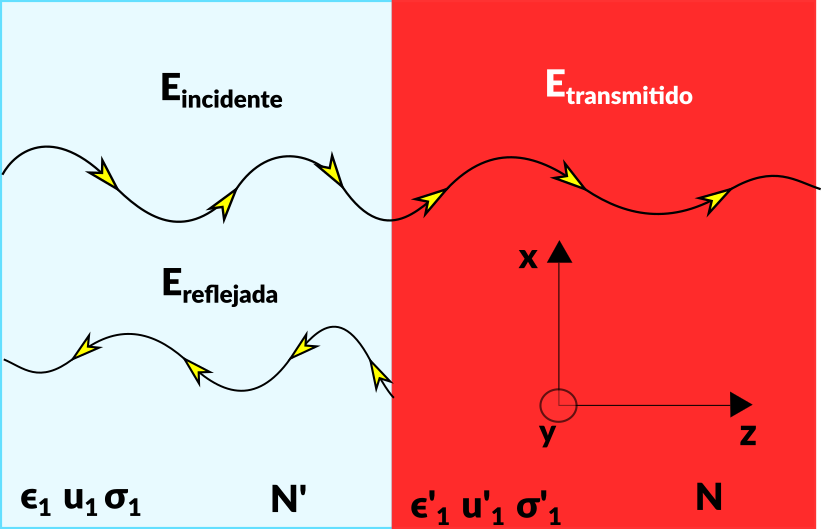
\includegraphics[width=0.85\textwidth]{reflectividadNormal.png}
\caption{Esquema de radiaci\'on a incidencia normal sobre una superficie: rayos incidente, reflejado y transmitido.}
\label{fig:incid-normal}
\end{figure}

\section{Transmitancia de una l\'amina}

Para una l\'amina de espesor $d$ en aire, sumando reflexiones m\'ultiples incoherentes,
\begin{equation}
\label{eq:T}
T=\frac{(1-R)^{2}x}{1-R^{2}x^{2}},
\qquad
x=e^{-\alpha d}=e^{-4\pi\tilde\nu k\,d},
\end{equation}
y la absorbancia decadica (densidad \'optica)
\begin{equation}
A=-\log_{10}T.
\end{equation}
Sin espesor no hay $T$ ni $A$ bien definidos desde el modelo.

\section{Funci\'on de p\'erdida}

La funci\'on de p\'erdida de energ\'ia
\begin{equation}
-\mathrm{Im}\!\left(\frac{1}{\hat\varepsilon}\right)
=\frac{\varepsilon_2}{\varepsilon_1^{2}+\varepsilon_2^{2}}
\end{equation}
resalta modos longitudinales y el plasm\'on.
Un $\varepsilon_\infty$ demasiado bajo infla artificialmente esta magnitud porque $|1/\varepsilon|$ crece.

\section{Procesos \'opticos en el s\'olido}

En distintos rangos espectrales dominan mecanismos distintos~\cite{MarkFox,Ashcroft}:
\begin{itemize}[leftmargin=*]
\item infrarrojo lejano y medio: fonones y portadores libres (Drude);
\item visible y ultravioleta cercano: transiciones interbanda, excitones;
\item energ\'ias a\'un mayores: contribuciones que, vistas desde una ventana limitada, se aglomeran en $\varepsilon_\infty$.
\end{itemize}

\begin{figure}[H]
\centering
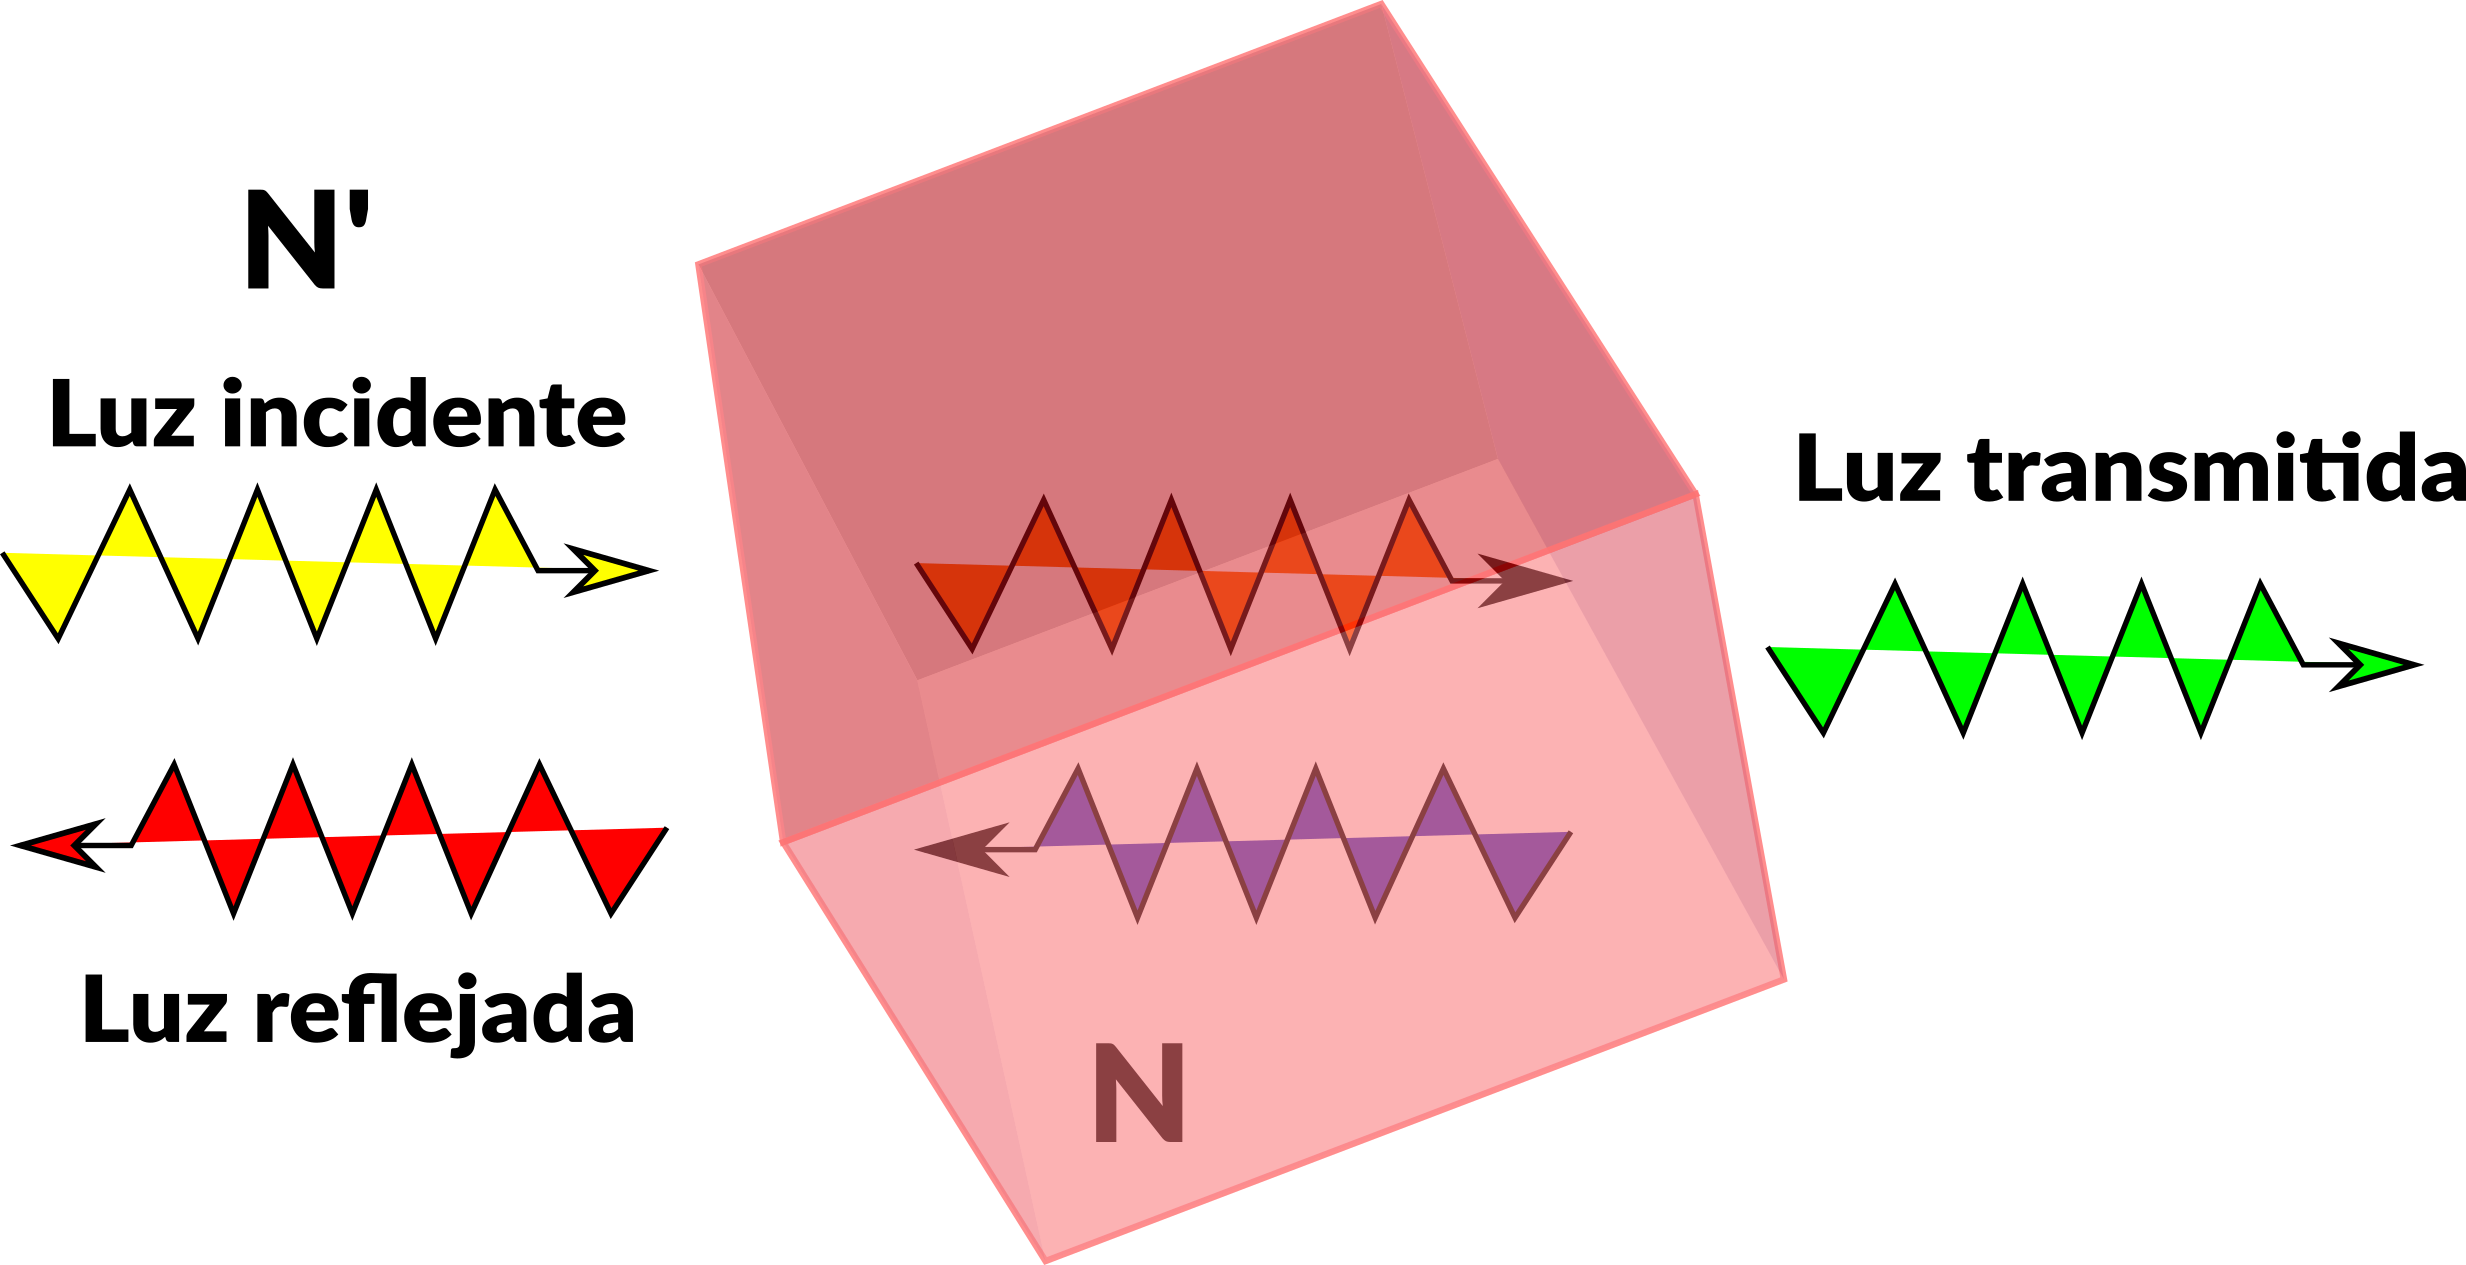
\includegraphics[width=0.88\textwidth]{procesosopticos.png}
\caption{Clasificaci\'on esquem\'atica de procesos \'opticos seg\'un la escala de energ\'ia.}
\label{fig:procesos}
\end{figure}

El modelo de Drude para electrones libres,
\begin{align}
\label{eq:drude}
\varepsilon_{2,\mathrm{D}}&=\frac{\omega_p^{2}\gamma\omega}{\omega^{4}+\gamma^{2}\omega^{2}},\\
\varepsilon_{1,\mathrm{D}}&=\varepsilon_\infty-\frac{\omega_p^{2}\omega^{2}}{\omega^{4}+\gamma^{2}\omega^{2}},
\end{align}
describe el fondo met\'alico.
En el an\'alisis variacional puede restarse antes de ajustar los tri\'angulos, de modo que las anclas describan el resto del espectro~\cite{constrained}.


\chapter{Causalidad y relaciones Kramers--Kronig}
\label{ch:kk}

\section{De la respuesta temporal a la frecuencia}

Si la polarizaci\'on es
\begin{equation}
\mathbf{P}(t)=\int_{-\infty}^{t}\chi(t-t')\,\mathbf{E}(t')\,dt',
\end{equation}
la funci\'on de respuesta $\chi(\tau)$ se anula para $\tau<0$.
En frecuencia, $\hat\varepsilon(\omega)=1+4\pi\hat\chi(\omega)$ es anal\'itica en el semiplano superior (con convenciones habituales), y las relaciones~\eqref{eq:kk1}--\eqref{eq:kk2} siguen del teorema de Cauchy~\cite{Jackson}.

\begin{figure}[H]
\centering
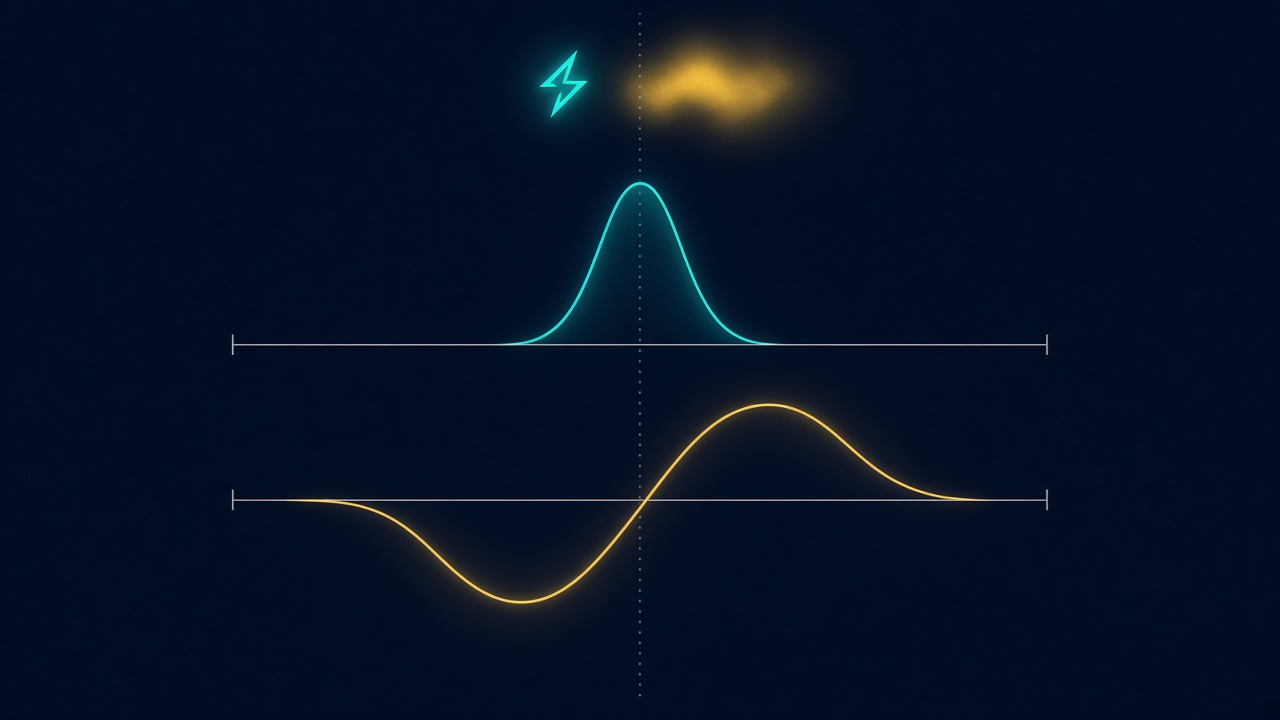
\includegraphics[width=0.82\textwidth]{learn-kk.jpg}
\caption{Un pico de absorci\'on en $\varepsilon_2$ fija la forma dispersiva de $\varepsilon_1$: no son dos ajustes independientes.}
\label{fig:kk-pair}
\end{figure}

\section{Ventana experimental y $\varepsilon_\infty$}

La integral Kramers--Kronig requiere, en principio, todo el eje.
En la pr\'actica se escribe
\begin{equation}
\label{eq:eps1-window}
\varepsilon_1(\omega)
=\varepsilon_\infty
+\frac{2}{\pi}\,\mathcal{P}\!\int_{\omega_{\min}}^{\omega_{\max}}
\frac{x\,\varepsilon_2(x)}{x^{2}-\omega^{2}}\,dx
+\text{(colas)},
\end{equation}
donde $\varepsilon_\infty$ recoge la contribuci\'on de altas frecuencias no medidas.
Interpretaci\'on operativa:
\begin{itemize}[leftmargin=*]
\item si el usuario fija $\varepsilon_\infty$, ese valor se respeta;
\item si se mide $n$ o $\varepsilon_1$, $\varepsilon_\infty$ puede ajustarse junto con las alturas de $\varepsilon_2$;
\item si se mide $R$ y $\varepsilon_\infty$ no se da, puede estimarse del extremo de alta frecuencia asumiendo $k$ peque\~no:
$n=(1+\sqrt{R})/(1-\sqrt{R})$, $\varepsilon_\infty=n^{2}$;
\item si se mide $k$, $\alpha$ o $T$, la magnitud no fija $\varepsilon_\infty$; el valor por defecto~$1$ reproduce bien $\alpha$ y $k$, pero no necesariamente $n$ ni $R$.
\end{itemize}

\section{Pasividad}

Un medio pasivo exige $\varepsilon_2(\omega)\ge 0$.
En el ajuste se puede penalizar $\varepsilon_2$ negativa para no abandonar el dominio f\'isico.
Esa penalizaci\'on es una regularizaci\'on f\'isica, no un dato experimental adicional.


\chapter*{Seminario I\\Respuesta \'optica lineal y la funci\'on diel\'ectrica}
\addcontentsline{toc}{chapter}{Seminario I}
\label{sem:1}

\noindent\textit{Parte~I --- exposici\'on de seminario.}

\section*{S.I.1 Prop\'osito}

Este seminario resume, para un auditorio de f\'isica de materiales, el contenido necesario antes de hablar de ajuste num\'erico:
qu\'e es $\hat\varepsilon$, c\'omo se conecta con lo que se mide, y por qu\'e Kramers--Kronig no es un adorno matem\'atico sino una ley de causalidad.

\section*{S.I.2 Mensaje central}

\begin{enumerate}[leftmargin=*]
\item Toda magnitud \'optica lineal de inter\'es puede escribirse en t\'erminos de $\varepsilon_1$ y $\varepsilon_2$ (o de $n$ y $k$).
\item Medir una sola proyecci\'on no basta, en general, para fijar el par completo sin hip\'otesis adicionales.
\item La causalidad suministra esa hip\'otesis: conocida $\varepsilon_2$ en un eje suficientemente amplio, $\varepsilon_1$ queda determinada salvo el fondo $\varepsilon_\infty$ de lo no medido.
\item Por tanto, el problema bien planteado es: \emph{buscar el $\varepsilon_2$ causal cuyo par Kramers--Kronig reproduce la magnitud experimental}.
\end{enumerate}

\section*{S.I.3 Demostraci\'on guiada (pizarra)}

\begin{enumerate}[leftmargin=*]
\item Partir de $\hat N^{2}=\hat\varepsilon$ y obtener~\eqref{eq:eps-nk}.
\item Invertir a~\eqref{eq:nk-from-eps}.
\item Sustituir en~\eqref{eq:R} y discutir el l\'imite transparente $k\to 0$.
\item Enunciar~\eqref{eq:kk1} e interpretar el pico de $\varepsilon_2$ frente a la dispersi\'on an\'omala de $\varepsilon_1$.
\item Se\~nalar el papel de $\varepsilon_\infty$ como ``todo lo que no cabe en la ventana''.
\end{enumerate}

\section*{S.I.4 Criterio de \'exito del seminario}

Al final, el auditorio debe poder responder sin ambig\"uedad:
\begin{itemize}[leftmargin=*]
\item qu\'e se gana al obtener $\hat\varepsilon$ frente a quedarse solo con $R$ o $\alpha$;
\item por qu\'e un ajuste independiente de $\varepsilon_1$ y $\varepsilon_2$ puede violar causalidad;
\item qu\'e hip\'otesis f\'isicas entran al estimar $\varepsilon_\infty$ desde $R$ en el extremo alto.
\end{itemize}

\section*{S.I.5 Puente hacia la Parte~II}

El Seminario~II tratar\'a c\'omo construir $\varepsilon_2$ con tri\'angulos, c\'omo evaluar $\varepsilon_1$ en forma cerrada y c\'omo minimizar $\chi^{2}$ sin abandonar Kramers--Kronig en ning\'un paso.
